%Chap 5 pag 29
\definecolor{Purple}{RGB}{153,0,153}
\definecolor{Pink}{RGB}{255,0,131}
\begin{frame}{Consistencia del arco}
La forma más simple de propagación hace que cada arco sea \textcolor{blue}{consistente}\\
\textcolor{Purple}{$X \longrightarrow Y$}\, es consistente si y solo si \\
por \textcolor{Pink}{cada} valor \textcolor{Purple}{x} de \textcolor{Purple}{$X$} hay \textcolor{Pink}{algunos} permitidos de \textcolor{Purple}{y}\\
\begin{figure}
    \centering
    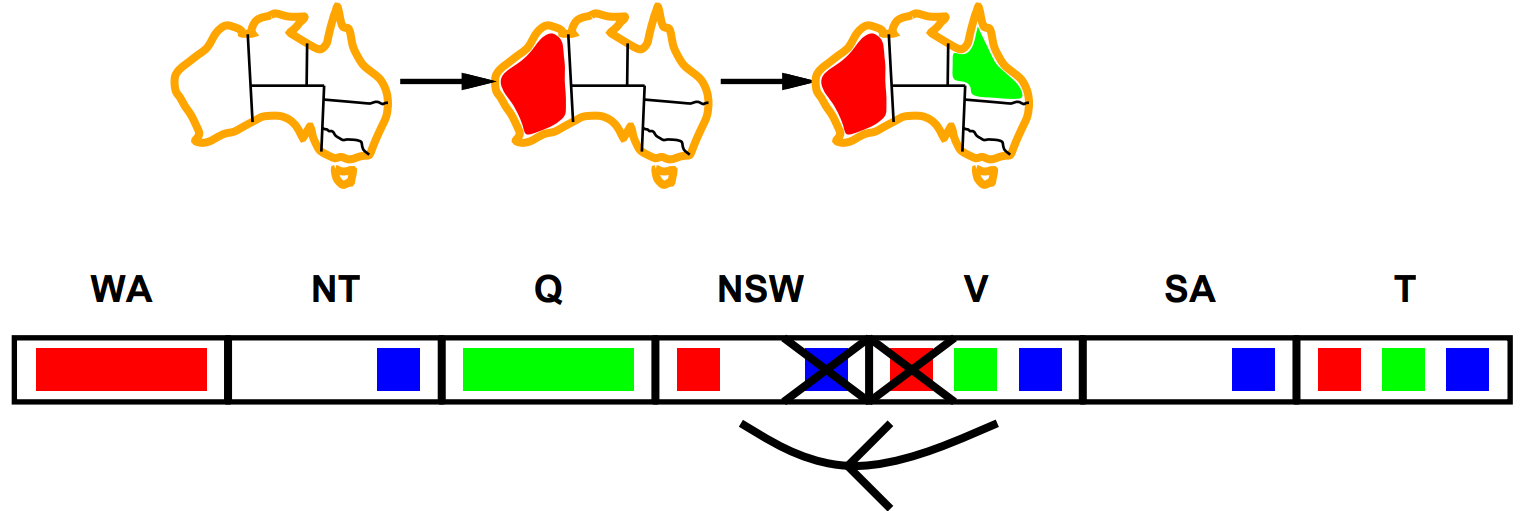
\includegraphics[width = 90mm, scale = 1]{images/29_5image.PNG}
\end{figure}
Si \textcolor{Purple}{X} pierde un valor, los vecinos de \textcolor{Purple}{X} deben volver a comprobarse\\
\end{frame}
